% !TEX program = uplatex
% !TEX encoding = UTF-8 Unicode
% =====================================================================
%  卒業論文発表スライド
%  題目 : 相関付きランダムウォークモデルを用いた時系列解析
%  発表 : 2520148K 北村 慎悟（愛媛大学 工学部 工学科 応用数理研究室）
%  指導 : 安藤 和典 教授・森岡 悠 准教授
%  仕様 : 発表7分 / 画面比率 16:9 / 日本語 / 発表者ノート付き
%
%  --- コンパイル方法（日本語 upLaTeX + dvipdfmx）----------------------
%    uplatex  presentation.tex
%    uplatex  presentation.tex      % 総ページ数・相互参照の確定に2回
%    dvipdfmx presentation.dvi
%    （platex でも可。ファイルは必ず UTF-8 で保存してください）
%
%  --- 図について ------------------------------------------------------
%    ../thesis/ 配下の PNG を参照します（\graphicspath で設定済み）。
%    画像が見つからない場合も \safeincludegraphics がプレースホルダを
%    表示するため，コンパイルは止まりません。
%
%  --- 発表者ノート ----------------------------------------------------
%    各フレーム直後の \note{...} が発表原稿です。合計の目安は約7分。
%      ・スライドのみ         : 既定（このまま）
%      ・ノートページ付き     : 下の \setbeameroption{show notes} を有効化
%      ・発表者ビュー(左右)   : show notes on second screen=right を有効化
%
%  --- おおよその時間配分（合計 約7分）--------------------------------
%    表紙 12s / 背景・目的 50s / RW→CRW 45s / 極限分布 42s /
%    予測モデル 48s / 離散化 38s / 実験(1) 52s / 実験(2) 40s /
%    限界 55s / まとめ 45s / 謝辞 8s
% =====================================================================
\documentclass[dvipdfmx,aspectratio=169,10pt]{beamer}

% ---- dvipdfmx で beamer を使うための補助（無い環境では読み飛ばす）----
\IfFileExists{bxdpx-beamer.sty}{\usepackage{bxdpx-beamer}}{}
\IfFileExists{pxjahyper.sty}{\usepackage{pxjahyper}}{}

\usepackage{amsmath,amssymb}
\usepackage{tikz}

% 日本語をゴシック体（サンセリフ相当）に統一
\ifdefined\kanjifamilydefault
  \renewcommand{\kanjifamilydefault}{\gtdefault}
\fi

% ---- 発表者ノートの表示切り替え（必要に応じてコメントを外す）--------
%\setbeameroption{show notes}
%\setbeameroption{show notes on second screen=right}

% ======================  配色・デザイン  =============================
\definecolor{myblue}{RGB}{23,54,93}     % 濃紺（基調色）
\definecolor{mygold}{RGB}{193,146,42}   % 金（アクセント：金価格にちなむ）
\definecolor{myaccent}{RGB}{150,95,0}   % 強調テキスト用の濃い琥珀
\definecolor{mygray}{RGB}{90,90,90}

\setbeamercolor{structure}{fg=myblue}
\setbeamercolor{title}{fg=myblue}
\setbeamercolor{frametitle}{fg=myblue}
\setbeamercolor{normal text}{fg=black}
\setbeamercolor{alerted text}{fg=myaccent}
\setbeamercolor{block title}{fg=white,bg=myblue}
\setbeamercolor{block body}{bg=myblue!8}
\setbeamercolor{itemize item}{fg=mygold}
\setbeamercolor{itemize subitem}{fg=mygold}
\setbeamercolor{enumerate item}{fg=myblue}
\setbeamercolor{author in head/foot}{fg=white,bg=myblue}
\setbeamercolor{title in head/foot}{fg=white,bg=myblue}

\setbeamerfont{frametitle}{size=\large,series=\bfseries}
\setbeamerfont{author in head/foot}{size=\scriptsize}
\setbeamerfont{title in head/foot}{size=\scriptsize}
\setbeamertemplate{navigation symbols}{}
\setbeamertemplate{itemize items}[circle]

% フレームタイトル：濃紺の見出し＋金の下線
\setbeamertemplate{frametitle}{%
  \vskip0.55em%
  {\usebeamercolor[fg]{frametitle}\usebeamerfont{frametitle}\insertframetitle\par}%
  \vskip0.12em%
  {\color{mygold}\rule{\textwidth}{1pt}}\par%
  \vskip0.15em%
}

% フッタ：題目（左）／氏名・ページ番号（右）
\setbeamertemplate{footline}{%
  \leavevmode%
  \hbox{%
    \begin{beamercolorbox}[wd=.62\paperwidth,ht=2.4ex,dp=1ex,leftskip=.35cm]{author in head/foot}%
      \usebeamerfont{author in head/foot}相関付きランダムウォークモデルを用いた時系列解析%
    \end{beamercolorbox}%
    \begin{beamercolorbox}[wd=.38\paperwidth,ht=2.4ex,dp=1ex,rightskip=.35cm]{title in head/foot}%
      \usebeamerfont{title in head/foot}\hfill 北村 慎悟\quad\insertframenumber\,/\,\inserttotalframenumber%
    \end{beamercolorbox}%
  }\vskip0pt%
}

% 画像が無くてもコンパイルを止めない安全な \includegraphics
\newcommand{\safeincludegraphics}[2][]{%
  \IfFileExists{#2}{\includegraphics[#1]{#2}}{%
  \IfFileExists{#2.pdf}{\includegraphics[#1]{#2.pdf}}{%
  \IfFileExists{#2.png}{\includegraphics[#1]{#2.png}}{%
  \IfFileExists{#2.jpg}{\includegraphics[#1]{#2.jpg}}{%
    \fbox{\begin{minipage}[c][32mm][c]{0.9\linewidth}\centering
      画像未配置\\[1mm]\texttt{\detokenize{#2}}
    \end{minipage}}%
  }}}}%
}

% 図はこのスライド専用に figures/ へコピー済み（Overleaf 等へも移植しやすい）。
% ../thesis/ 側も探索対象に含めているので，元図に差し替えても参照できる。
\graphicspath{{figures/}{./}{../thesis/}{../thesis/patterns_extra/}}

% =====================================================================
\begin{document}

% ============================  表紙  ================================
\begin{frame}[plain]
  \centering
  \vfill
  {\color{mygold}\rule{0.9\textwidth}{2.5pt}}\par\vskip1.1em
  {\usebeamercolor[fg]{title}\LARGE\bfseries 相関付きランダムウォークモデルを用いた\\[4pt]時系列解析\par}
  \vskip0.7em
  {\color{mygray}\large ―― 金価格の時系列予測への応用とモデルの限界 ――\par}
  \vskip0.6em
  {\color{mygold}\rule{0.9\textwidth}{2.5pt}}\par
  \vskip1.7em
  {\large 発表者\quad 2520148K\quad 北村 慎悟\par}
  \vskip0.5em
  {\normalsize 指導教員\quad 安藤 和典 教授\quad ・\quad 森岡 悠 准教授\par}
  \vskip0.9em
  {\small 愛媛大学 工学部 工学科（応用数理研究室）\par}
  \vskip0.2em
  {\small 2026年\quad 卒業論文発表会}% ← 発表日は適宜変更してください
  \vfill
\end{frame}
\note{% 【約12秒】
それでは発表を始めます。「相関付きランダムウォークモデルを用いた時系列解析」という題目で，応用数理研究室の北村慎悟が発表いたします。本研究では，相関付きランダムウォークという確率モデルを金価格の時系列予測に応用し，その妥当性と限界を実証的に調べました。よろしくお願いいたします。%
}

% =====================  1. 背景と目的  ==============================
\begin{frame}[t]{研究の背景と目的}
  \small
  \begin{block}{背景}
    \begin{itemize}
      \item 金（XAUUSD）はインフレや地政学的リスクを映す重要資産であり，値動きのモデル化への関心は高い
      \item \alert{相関付きランダムウォーク}\dots 直前の値動きの向きに応じて次の向きを確率的に決めるモデル。\alert{持続性・反転傾向を少数のパラメータで表現}できる
      \item Konno (2019) の\alert{量子ウォークによる時系列モデル}を，相関付きランダムウォークへ応用したもの
      \item 金価格への適用は，筆者の知る限り先行研究が存在しない
    \end{itemize}
  \end{block}
  \begin{block}{目的}
    \begin{itemize}
      \item 金価格 XAUUSD を\alert{平均練行足}で $\pm1$ の系列へ離散化し，本モデルで次時刻を予測
      \item 予測と実測の\alert{重ね描き}と\alert{平均絶対誤差 (MAE)}により，記述の\alert{妥当性と限界}を実証的に検討
    \end{itemize}
  \end{block}
\end{frame}
\note{% 【約50秒】
まず研究の背景です。金はインフレや地政学的リスクを反映する重要な資産で，その値動きのモデル化には実務・学術の両面で関心があります。本研究で用いる相関付きランダムウォークは，直前の値動きの向きに応じて次の向きを確率的に決めるモデルで，値動きの持続性や反転傾向を，少数のパラメータで表現できます。これは，Konno が2019年に提案した量子ウォークによる時系列モデルを，相関付きランダムウォークに応用したものです。ただし，これを金価格に当てはめた先行研究は，私の知る限りありません。そこで本研究では，金価格 XAUUSD を平均練行足で離散化してこのモデルを当てはめ，予測と実測を重ねた図と MAE によって，妥当性と限界を検討します。%
}

% =================  2. RW と 相関付きRW  ============================
\begin{frame}[t]{ランダムウォークと相関付きランダムウォーク}
  \small
  \begin{columns}[T]
    \begin{column}{0.48\textwidth}
      {\color{myblue}\bfseries 通常のランダムウォーク}
      \begin{itemize}
        \item 各ステップは\alert{独立}に $\pm1$
        \item 位置 $\displaystyle S_n=\sum_{k=1}^{n} T_k$
        \item 直前の向きは次の一歩に\alert{無関係}
      \end{itemize}
    \end{column}
    \begin{column}{0.48\textwidth}
      {\color{myblue}\bfseries 相関付きランダムウォーク}
      \begin{itemize}
        \item 直前の向きが次の向きの確率に\alert{影響}
        \item $P(\text{左}\mid\text{直前左})=a,\ P(\text{右}\mid\text{直前右})=d$
        \item コイン行列 $A=\begin{pmatrix}a&b\\c&d\end{pmatrix}$\, ($a{+}c{=}b{+}d{=}1$)
      \end{itemize}
    \end{column}
  \end{columns}
  \vskip0.7em
  \begin{block}{持続性と反転傾向（時間発展対称 $a=d$，$A=\left(\begin{smallmatrix}a&1-a\\1-a&a\end{smallmatrix}\right)$）}
    \begin{itemize}
      \item $a>\tfrac12$：同じ向きに進みやすい＝\alert{持続性}／$a<\tfrac12$：向きが反転しやすい＝\alert{反転傾向}
      \item 左右の移動行列 $P,Q$ は\alert{非可換} $\Rightarrow$ 移動の順序が違えば確率も変わる（通常RWとの本質的な違い）
    \end{itemize}
  \end{block}
\end{frame}
\note{% 【約45秒】
次にモデルの定義です。通常のランダムウォークは，各ステップが独立にプラス1かマイナス1動くもので，直前にどちらへ動いたかは，次の一歩に影響しません。一方，相関付きランダムウォークでは，直前の向きが次の向きの確率に影響します。左のあとに左へ進む確率を $a$，右のあとに右へ進む確率を $d$ とし，これらをまとめたものがコイン行列 $A$ です。特に $a=d$ のときを時間発展対称とよびます。$a$ が2分の1より大きいと，同じ向きに進みやすい持続性を，小さいと向きが反転しやすい反転傾向を表します。なお，左右の移動を表す行列は非可換で，同じ移動回数でも動く順序が違えば確率が変わる点が，通常のランダムウォークとの本質的な違いです。%
}

% =====================  3. 極限分布  ===============================
\begin{frame}[t]{相関付きランダムウォークの性質：極限分布}
  \small
  \begin{columns}[T]
    \begin{column}{0.44\textwidth}
      \begin{itemize}
        \item 弱収束極限定理：
          \[ \frac{\tilde S_n}{\sqrt n}\ \Rightarrow\ N\!\left(0,\ \tfrac{a}{1-a}\right) \]
        \item 分散 $\sigma^2=\dfrac{a}{1-a}$
          \begin{itemize}\footnotesize
            \item $a=\tfrac12$：$\sigma^2=1$（通常RWと一致）
            \item $a>\tfrac12$（持続性）：$\sigma^2>1$，\alert{裾が広い}
            \item $a<\tfrac12$（反転）：$\sigma^2<1$，\alert{裾が狭い}
          \end{itemize}
        \item \alert{たった1つの $a$} で値動きの粘り／反発を表現できる
      \end{itemize}
    \end{column}
    \begin{column}{0.56\textwidth}
      \centering
      \safeincludegraphics[width=\linewidth]{figures/crw_hist_n100}
      \par{\footnotesize\color{mygray}$n=100$ の分布と標準正規分布の比較}
    \end{column}
  \end{columns}
\end{frame}
\note{% 【約42秒】
このモデルの性質を，極限分布で見ます。時刻 $n$ の位置をルート $n$ で割ると，平均0，分散 $a$ 割る $1{-}a$ の正規分布に弱収束します。分散は $a$ が2分の1のとき1，つまり通常のランダムウォークと一致し，$a$ が大きいほど大きく，小さいほど小さくなります。図は $n=100$ での分布を標準正規分布と比べたものです。持続性を持つ $a=3$ 分の2の濃い分布は，中央が低く裾が広がり，反転傾向を持つ $a=3$ 分の1の薄い分布は，中央が高く裾が狭くなっています。このように，たった一つのパラメータ $a$ で，値動きの粘りや反発の強さを表せることが，このモデルの特徴です。%
}

% =====================  4. 予測モデル  =============================
\begin{frame}[t]{相関付きランダムウォークによる時系列予測モデル}
  \small
  \begin{block}{手順（Konno の量子ウォーク時系列モデルを相関付きRWへ応用）}
  \begin{enumerate}
    \item 観測値を，増分 $b_n=x_n-x_{n-1}\in\{-1,+1\}$，$x_0=0$ の系列で表す
    \item モデルの位置確率 $\mu_t(x;p,q,\alpha)=P(\tilde S_t=x)$
      \\{\footnotesize（$p$：右継続確率，$q$：左継続確率，$\alpha$：初期が左向きの確率）}
    \item \alert{評価関数}（観測 $x_t$ とモデル位置 $x$ の二乗誤差を，確率で重み付け）
      \[ V_n(p,q,\alpha)=\sum_{t=0}^{n}\sum_{x=-t}^{t}(x-x_t)^2\,\mu_t(x;p,q,\alpha) \]
    \item $V_n$ を最小化するパラメータ $(p^\ast,q^\ast,\alpha^\ast)$ を格子上の全探索で推定
    \item \alert{次時刻を期待値で予測}\quad
      $x_{n+1}^{\ast}=E\!\left(\tilde S_{n+1}\mid p^\ast,q^\ast,\alpha^\ast\right)$
  \end{enumerate}
  \end{block}
\end{frame}
\note{% 【約48秒】
では，このモデルをどう予測に使うかです。まず，観測した値動きを，増分がプラス1かマイナス1の系列として表します。モデルは，パラメータ $p$，$q$，$\alpha$ で，時刻 $t$ に位置 $x$ にいる確率 $\mu$ を与えます。$p$ は右への継続確率，$q$ は左への継続確率，$\alpha$ は初期の向きが左である確率です。次に，観測値 $x$ と，モデルが取りうる位置 $x$ との二乗誤差を，その位置の確率で重み付けして足し合わせた，評価関数 $V$ を作ります。これを最小にするパラメータを，格子上の全探索で推定し，そのパラメータのもとでの次時刻の期待値を，予測値とします。これが，Konno の量子ウォーク時系列モデルを，相関付きランダムウォークに応用した予測の枠組みです。%
}

% =====================  5. 離散化  ================================
\begin{frame}[t]{金価格データの離散化：平均練行足}
  \small
  \begin{columns}[T]
    \begin{column}{0.52\textwidth}
      \begin{itemize}
        \item XAUUSD：ドル建ての金価格（1トロイオンス）
        \item 連続的な価格を\alert{値幅 $B$ ごとの上昇・下降（$\pm1$）}へ変換
          \begin{itemize}\footnotesize
            \item $P_t\ge o_i+B$ なら $+1$（基準を $+B$ 更新）
            \item $P_t\le o_i-B$ なら $-1$（基準を $-B$ 更新）
            \item 継続でも反転でも $B$ 動けば1本生成
          \end{itemize}
        \item 符号を累積 $\displaystyle x_n=\sum_{k=1}^{n}b_k$ し，\alert{ボックス単位の整数時系列}を得る
        \item この離散系列をモデルの入力とする
      \end{itemize}
    \end{column}
    \begin{column}{0.46\textwidth}
      \centering
      \resizebox{\linewidth}{!}{%
      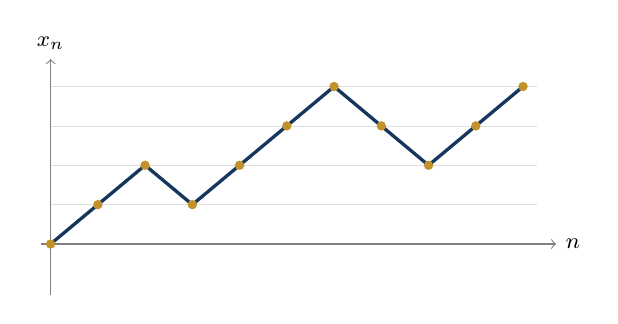
\begin{tikzpicture}[x=0.60cm,y=0.50cm,line join=round]
        \draw[->,gray] (-0.2,0)--(10.7,0) node[right,black]{\footnotesize $n$};
        \draw[->,gray] (0,-1.3)--(0,4.7) node[above,black]{\footnotesize $x_n$};
        \foreach \y in {1,2,3,4} \draw[gray!25,very thin] (0,\y)--(10.3,\y);
        \draw[very thick,myblue]
          (0,0)--(1,1)--(2,2)--(3,1)--(4,2)--(5,3)--(6,4)--(7,3)--(8,2)--(9,3)--(10,4);
        \foreach \x/\y in {0/0,1/1,2/2,3/1,4/2,5/3,6/4,7/3,8/2,9/3,10/4}
          \fill[mygold] (\x,\y) circle (1.7pt);
      \end{tikzpicture}}
      \par\vskip0.4em{\footnotesize\color{mygray}$\pm1$ を積み上げた整数時系列 $x_n$ の例}
    \end{column}
  \end{columns}
\end{frame}
\note{% 【約38秒】
実際の金価格は連続的に変動するので，そのままではモデルに入れられません。そこで，平均練行足という手法で，値幅 $B$ ごとの上昇・下降に変換します。基準価格から $B$ 以上上がればプラス1の足，$B$ 以上下がればマイナス1の足を立て，継続でも反転でも $B$ 動けば1本生成します。大きく動いた場合は，同じ向きに複数本立てます。こうして得た符号を積み上げると，図のような，ボックス単位の整数の時系列 $x$ になります。この離散化された系列を，先ほどのモデルの入力として使います。%
}

% =================  6. 実験(1)：全期間参照  ========================
\begin{frame}[t]{実験①：全期間参照とその失敗}
  \small
  \begin{block}{実験設定}
    \begin{itemize}\footnotesize
      \item データ：XAUUSD 1分足（2026-06-29〜30，UTC，317本），値幅 $B=3$ ドル，練行足 $N=156$ 本
      \item 評価：\alert{予測と実測の重ね描き}を中心に，補助指標として MAE と方向的中率 HIT
      \item 目安：練行足は毎回 $\pm1$ 動くため，「変化なし」予測は $\mathrm{MAE}=1$，でたらめな方向予測は $\mathrm{HIT}=0.5$
    \end{itemize}
  \end{block}
  \begin{block}{全期間 $D_n$ を参照した場合（第5章のモデルそのまま）}
    \begin{itemize}
      \item \alert{$\mathrm{MAE}=5.94$}（基準の約6倍），\alert{$\mathrm{HIT}=0.43$}（$0.5$ 未満）→ 両指標で基準以下
      \item 原因：全期間参照は値動きを\alert{定常}と仮定。実際は\alert{非定常}（上昇・下降・レンジが移り変わる）ため，終わった局面の観測が推定に混入し，予測が系統的にずれる
    \end{itemize}
  \end{block}
\end{frame}
\note{% 【約52秒】
ここから実験結果です。対象は XAUUSD の1分足で，2026年6月末の約5時間，値幅 $B$ は3ドル，練行足は156本です。評価は，予測と実測を重ねた図を中心に，補助としてMAEと方向的中率HITを使います。練行足は毎回必ずプラスマイナス1動くので，変化なし予測のMAEは1，方向をでたらめに当てるHITは0.5が目安になります。まず，第5章のモデルをそのまま，過去の全期間を参照して当てはめると，MAEは5.94と基準の約6倍，HITは0.43と0.5を下回り，両方の指標で基準を下回りました。原因は，全期間参照が値動きを定常と仮定している点にあります。実際の価格は，上昇・下降・レンジが移り変わる非定常な系列なので，終わった局面の観測が推定に混ざり続け，予測が系統的にずれてしまうのです。%
}

% =================  7. 実験(2)：参照期間W  =========================
\begin{frame}[t]{実験②：参照期間 $W$ の導入と効果}
  \small
  \begin{columns}[T]
    \begin{column}{0.44\textwidth}
      \begin{itemize}
        \item 改良：当てはめを\alert{直近 $W$ 点}に限定（参照期間 $W$）
        \item $W\in\{2,3,5,10,20,30,60,\text{全期間}\}$ を比較
        \item MAE は\alert{$W$ が小さいほど小さい}
          \begin{itemize}\footnotesize
            \item 最小は $W=2$ で $\mathrm{MAE}=0.847$
            \item 基準 $1$ を下回るのは $W=2,\,3$ のみ
          \end{itemize}
        \item 計算時間も $W$ とともに増加
        \item \alert{精度と計算量にトレードオフなし}（小さい $W$ が両面で有利）
      \end{itemize}
    \end{column}
    \begin{column}{0.56\textwidth}
      \centering
      \safeincludegraphics[width=\linewidth]{figures/w_sweep_summary}
      \par{\footnotesize\color{mygray}参照期間 $W$ に対する MAE（左）と1ステップ計算時間（右）}
    \end{column}
  \end{columns}
\end{frame}
\note{% 【約40秒】
そこで，当てはめに使う観測を，直近の $W$ 点だけに絞る，参照期間 $W$ を導入します。$W$ を2から全期間まで変えて比較したのが，この図です。左のMAEを見ると，$W$ が小さいほど誤差が小さく，$W=2$ で最小の0.847になります。基準の1を下回るのは，$W=2$ と $W=3$ だけでした。右の計算時間も，$W$ とともに増えます。つまり，精度と計算量の間にトレードオフはなく，参照期間を小さく絞るほど，誤差も計算量も小さくなるという，一見望ましい結果が得られました。%
}

% =====================  8. モデルの限界  ==========================
\begin{frame}[t]{モデルの限界：局面転換への追従の遅れ}
  \small
  \begin{columns}[T]
    \begin{column}{0.54\textwidth}
      \centering
      \safeincludegraphics[width=\linewidth]{figures/pat_up2down_w}
      \par{\footnotesize\color{mygray}上昇→下降の局面（合成データ，$N=150$）}
    \end{column}
    \begin{column}{0.44\textwidth}
      \begin{itemize}\footnotesize
        \item 大きい $W{=}60$ は転換点を過ぎても上昇の勢いを引きずり，実測から大きく乖離
          （\alert{$\mathrm{MAE}\,4.876$} vs $W{=}2$ の $0.892$）
        \item 機構：予測は\alert{参照期間の先頭から $W$ 歩後の期待値}であり，\alert{現在位置・直前の向きを条件づけない}
          \begin{itemize}\scriptsize
            \item $W$ 大 → 起点が遠く誤差増，かつ転換に $W$ 本の遅れ
          \end{itemize}
        \item \alert{「$W{=}2$ が最良」は精度の証明ではない}：履歴を使うほど誤差を上乗せする構造の下で，履歴をほぼ使わず悪化を最小化しただけ
        \item HIT は $W$ によらず約 $0.5$ → 方向を安定して当ててはいない
      \end{itemize}
    \end{column}
  \end{columns}
\end{frame}
\note{% 【約55秒】
しかし，この結果はモデルの優秀さを意味しません。図は，上昇から下降へ転じる局面です。参照期間の大きい $W=60$ は，転換点を過ぎても上昇の勢いを引きずり，実測から大きく乖離して，MAEは4.876，$W=2$ の0.892の5倍以上に悪化しています。原因はモデルの構造です。この予測は，参照期間の先頭から $W$ 歩後の期待値を求めるだけで，現在位置や直前の向きで条件づけていません。だから $W$ が大きいほど，起点が現在から遠くなって誤差が増え，局面が変わっても $W$ 本ぶんの遅れが出ます。つまり，$W=2$ が最良なのは，履歴を使うほど誤差を上乗せするこの構造のもとで，履歴をほとんど使わないことで，悪化を最小に抑えただけ，と見るべきです。実際，方向的中率HITは $W$ によらずおよそ0.5にとどまり，次の向きを安定して当てられてはいません。%
}

% =====================  9. まとめ  ================================
\begin{frame}[t]{まとめと今後の課題}
  \small
  \begin{block}{まとめ}
    \begin{itemize}
      \item 相関付きランダムウォーク（Konno 型時系列モデル）を，金価格 XAUUSD に\alert{平均練行足}を通して初めて適用
      \item 全期間参照は破綻（$\mathrm{MAE}=5.94$）。\alert{参照期間 $W$} の導入で改善し，$W=2$ で最良（$\mathrm{MAE}=0.847$）
      \item ただしこれは\alert{現在位置・向きを使わない構造的限界の裏返し}であり，履歴を活用するほど劣化する
    \end{itemize}
  \end{block}
  \begin{block}{今後の課題}
    \begin{itemize}\footnotesize
      \item 現在位置・直前の向きを\alert{条件づける}予測への拡張（条件付き期待値）
      \item 金以外の資産（株・為替・暗号資産・他商品）への適用
      \item 平均練行足に依らない離散化・非一定増分への拡張
      \item マルコフ連鎖・高次モデル・レジーム転換モデルとの比較
    \end{itemize}
  \end{block}
\end{frame}
\note{% 【約45秒】
まとめます。本研究では，相関付きランダムウォークによる時系列モデルを，金価格に，平均練行足を通して初めて適用しました。全期間参照ではMAEが5.94と破綻しましたが，参照期間 $W$ の導入で改善し，$W=2$ で最良の0.847が得られました。ただしこれは，現在位置や向きを予測に使わないという，構造的な限界の裏返しでもあります。今後の課題としては，現在位置と直前の向きを条件づける予測への拡張，金以外の資産への適用，平均練行足に依らない離散化への拡張，そして，マルコフ連鎖など他のモデルとの比較が挙げられます。以上です。%
}

% =====================  謝辞・結び  ===============================
\begin{frame}[plain]
  \centering\vfill
  {\color{mygold}\rule{0.6\textwidth}{2pt}}\par\vskip1.2em
  {\usebeamercolor[fg]{title}\Large\bfseries ご清聴ありがとうございました}\par
  \vskip1.0em
  {\color{mygray}\small 相関付きランダムウォークモデルを用いた時系列解析\\[2pt]2520148K\quad 北村 慎悟}\par
  \vskip1.0em
  {\color{mygold}\rule{0.6\textwidth}{2pt}}
  \vfill
\end{frame}
\note{% 【約8秒】
以上で発表を終わります。ご清聴ありがとうございました。%
}

\end{document}
